\documentclass{beamer}
\input{../../preamble}
\usecolortheme{crane}
\usepackage{eurosym}
\usepackage{hyperref}
\hypersetup{colorlinks=true}
\newcommand{\pblock}{\\ \vspace{0.5cm}\pause}
\newcommand{\socrativeOhje}{
\begin{itemize}
\item Surffaa osoitteeseen \url{m.socrative.com} (tai \url{socrative.com})
\item Siirry huoneeseen nimeltä \url{hruoho}
\end{itemize}
}

\newcommand{\taukoKysymys}{
\socrativeOhje
	\begin{block}{Kysymys}
	Mielestäni tähän väliin täydellinen tauko on
	\begin{enumerate}[(A)]
		\item 10 min
		\item 20 min
		\item 30 min
		\item Vähemmän 
		\item Enemmän
	\end{enumerate}	
	\end{block}
}
\title{Talousmatematiikkaa: verotus}
\begin{document}

\begin{frame}
\maketitle
\end{frame}
\begin{frame}
\tableofcontents
\end{frame}
\begin{frame}

\socrativeOhje
\begin{block}{Kysymys}
Haluaisin, että
\begin{enumerate}[(A)]
\item prosenttilaskenta kerrattaisiin kunnolla (10min)
\item prosenttilaskennasta katsottaisiin esimerkki
\item prosenttilaskennan kertaaminen sivuutettaisiin
\end{enumerate}
\end{block}
\end{frame}

\section{Prosenttilaskentaa}
\begin{frame}
\frametitle{Prosenttiosuuden laskeminen}
	\begin{esim}
		Tuotteen myyntihinta oli 119,90 euroa. 
		\begin{enumerate}[(a)]
			\item Hintaa laskettiin 20\%. Laske alennus ja uusi hinta.
			\item Hintaa korotettiin myöhemmin 20\%. Laske korotuksen suuruus. Miten viimeisin hinta suhtautuu alkuperäiseen?
		\end{enumerate}
	\end{esim}
\end{frame}
\begin{frame}
	\begin{ratkaisu}
		\begin{enumerate}[(a)]
			\item Alennus on 20\% alkuperäisestä hinnasta\pause , eli 
			\[
			0,20\cdot119,90 = 23,98
			\] euroa. \pause Näin ollen uusi hinta on 
			\[
			119,90-23,98 = 95,92
			\] euroa. \pause (Toisaalta uusi hinta on 80\% alkuperäisestä hinnasta, eli \(
			0,80\cdot 119,90 = 95,92\) euroa.)
			\item \pause Uusi hinta on 120\% edellisestä hinnasta\pause , eli
			\[
			1,20\cdot95,92\approx 115,10
			\] euroa. \pause Uusi hinta on siis 4,80 euroa pienempi kuin alkuperäinen.
		\end{enumerate}
	\end{ratkaisu}
\end{frame}

\begin{frame}
\frametitle{Prosenttiluvun laskeminen}
	\pause 
	\begin{esim}
		Kahvilassa kävi päivän aikana 34 mies- ja 48 naisasiakasta. Kuinka suuri osa asiakkaista oli miehiä? Entä naisia?
	\end{esim}
	\pause
	\begin{ratkaisu}
		Asiakkaita oli yhteensä 82 kpl. \pause Miesten osuus oli
		\[
			\frac{34}{82} \approx 0,415 = 41,5\%
		\]
		\pause
		ja naisten osuus
		\[
			\frac{48}{82} \approx 0,585 = 58,5 \%
		\]
		
	\end{ratkaisu}
\end{frame}

\begin{frame}
\frametitle{Perusarvon laskeminen}
	\begin{esim}
		Takki myytiin 30\% alennuksella hintaan 140 euroa. Laske alkuperäinen hinta.
	\end{esim}
	\begin{ratkaisu}
		Olkoon \(x\) alkuperäinen hinta.\pause Tällöin alennettu hinta on \(0,70x\)\pause , joten
		\[
			0,70x = 140
		\]
		\pause Tästä saadaan \(x=200\). \pause Siis alkuperäinen hinta oli 200 euroa.
	\end{ratkaisu}
\end{frame}

% Onko tarvetta?
%
%\begin{frame}
%\frametitle{Muutos- ja vertailuprosentti}
%\end{frame}

\section{Arvonlisävero}

\begin{frame}
\frametitle{Arvonlisävero}
\pause
Lähes kaikkien Suomessa myytävien tuotteiden ja palveluiden hinnat sisältävät arvonlisäveron
\pblock
Arvonlisävero on tarkoitettu kuluttajan maksettavaksi
\pblock
Suomessa on käytössä neljä \href{http://www.veronmaksajat.fi/luvut/tilastot/kulutusverot/arvonlisavero/}{arvonlisäverokantaa}
\pblock
Arvonlisävero tilitetään valtiolle myyjän toimesta
\end{frame}

\begin{frame}
\frametitle{Arvonlisävero}
\pause
\begin{figure}
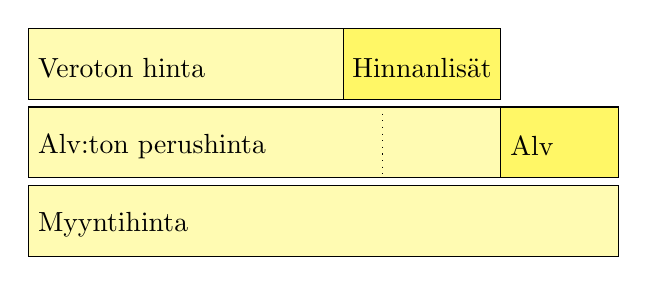
\begin{tikzpicture}
	%veroton hinta
	\draw[fill=yellow, fill opacity=0.3](-3,0.1) rectangle (1,1);
	%hinnanlisät
	\draw[fill=yellow, fill opacity=0.6](1,0.1) rectangle (3,1);
	%perushinta
	\draw[fill=yellow, fill opacity=0.3](-3,-0.9) rectangle (3,0);
	\draw[dotted] (1.5,0)--(1.5,-0.9);
	%alv	
	\draw[fill=yellow, fill opacity=0.6](3,-0.9) rectangle (4.5,0);
	%myyntihinta
	\draw[fill=yellow, fill opacity=0.3](-3,-1.9) rectangle (4.5,-1);
	\draw(-3,0.5) node[right]{Veroton hinta};
	\draw(2,0.5) node{Hinnanlisät};
	\draw(-3,-0.5) node[right]{Alv:ton perushinta};
	\draw(3,-0.5) node[right]{Alv};
	\draw(-3,-1.5) node[right]{Myyntihinta};
\end{tikzpicture}
\caption{Arvonlisävero (alv) lasketaan alv:ttomasta perushinnasta}
\end{figure}
\end{frame}



\begin{frame}
\frametitle{Arvonlisäveron laskeminen}
	\begin{itemize}
		\item \(P =\) perushinta eli arvonlisäveroton hinta
		\item \(i =\) veroprosentti (verokanta) desimaalilukuna ilmoitettuna (\(0 < i < 1\))
		\item \(M =\) myyntihinta eli verollinen hinta: \(M = P + ALV\)
		\item \(ALV =\) arvonlisäveron määrä euroina:
			\[
				ALV = i \cdot P\qquad\text{ tai }\qquad ALV = \frac{i}{1 + i}\cdot M
			\]
		\item Perushinnan ja myyntihinnan yhteys:
			\[
				M = (1 + i) \cdot P \qquad\text{ ja }\qquad P = \frac{M}{1 + i}
			\]
	\end{itemize}
\end{frame}

\begin{frame}
\frametitle{Arvonlisävero}
	\begin{esim}
		Tuotteen alv:ton hinta on 54,50 euroa. Laske myyntihinta, kun tuote kuuluu 24\% arvonlisäveron piiriin.
	\end{esim}
	\pause
	\begin{ratkaisu}
		Myyntihinta saadaan suoraan alv:ttomasta hinnasta: myyntihinta on 			\[
				1,24\cdot 54,50 = 67,58
			\] euroa.
	\end{ratkaisu}
\end{frame}


\begin{frame}
\frametitle{Arvonlisävero}
	\begin{esim}
		Tuotteen alv:ton hinta on 24,80 euroa ja myyntihinta 28,27 euroa. Minkä alv-kannan piiriin tuote kuuluu?
	\end{esim}
	\pause
	\begin{ratkaisu}
		Myyntihinta sisältää veroa  \(28,27-24,80 = 3,47\) euroa.\pause
		Veron osuus \emph{alv:ttomasta} hinnasta on 
		\[
			\frac{3,47}{24,8} \approx 0,14
		\]
		\pause
		Tuote kuuluu siis 14\% arvonlisäveron piiriin.
	\end{ratkaisu}
\end{frame}

\begin{frame}
\frametitle{Arvonlisävero}
	\begin{esim}
		Tuotteen myyntihinta on 133,00 euroa. Laske arvonlisäveron suuruus, kun tuote kuuluu 24\% arvonlisäveron piiriin.
	\end{esim}
	\pause
	\begin{ratkaisu}
		Olkoon \(x\) tuotteen alv:ton hinta. \pause Silloin \(x= 133/1,24\). \pause Niinpä veron suuruus on \pause
		\[
			133- x = 133 - \frac{133}{1,24}\approx 25,74
		\]
		euroa. \pause Tämä voitaisiin laskea myös suoraan kaavalla: arvonlisäveron suuruus on \pause
			\[
				\frac{0,24}{1,24}\cdot133,00\approx 25,74
			\]
		euroa.
	\end{ratkaisu}
\end{frame}

\begin{frame}
\frametitle{Arvonlisävero}
	\begin{esim}
		Viinipullon (0,7l) myyntihinta 21,90\euro\ sisältää alkoholiveroa 339,00 snt/litra ja arvonlisäveroa 24\%. Laske kyseisen viinin
		\begin{enumerate}[(a)]
			\item alv:ton litrahinta
			\item veroton litrahinta
		\end{enumerate}
	\end{esim}
\end{frame}


\begin{frame}
\frametitle{Arvonlisävero}

	\begin{ratkaisu}
		\pause
		\begin{enumerate}[(a)]
			\item \emph{Viinipullon} alv:ton hinta on\pause 
				\[
					\frac{21,90}{1,24}\approx 17,66
				\]
				euroa. \pause Näin ollen viinilitran alv:ton hinta on 
				\[
					\frac{17,66}{0,7}\approx 25,23
				\] euroa.\pause
			\item Edellisen perusteella viinilitran alkoholiveroton hinta olisi \pause
				\[
					25,23-\frac{339,00}{100} = 21,84
				\]
				euroa.
		\end{enumerate}
	\end{ratkaisu}
\end{frame}

\begin{frame}
\frametitle{Arvonlisävero myyntiketjussa}

Tuotteen jokaisessa jälleenmyyntivaiheessa tilitetään myytäessä saadun ja  ostettaessa maksetun arvonlisäveron erotus\pause
\begin{esim}
Jälleenmyyjä ostaa tuotteita ja maksaa ostaessaan arvonlisäveroa 1000 euroa. \pause Myöhemmin hän myy tuotteet ja saa myydessään arvonlisäveroa 1500 euroa. \pause Myyjä tilittää valtiolle arvonlisäverojen erotuksen \(1500-1000=500\) euroa. 
\end{esim}\pause
Arvonlisäveroa maksetaan tuotteen lisääntyneestä arvosta: arvonlisästä
\end{frame}

\begin{frame}
\taukoKysymys
\end{frame}

\section{Tuloverotus}

\begin{frame}
\frametitle{Tuloverotus}
\pause
Tuloverotus jaetaan ansio- ja pääomatulojen verotukseen
\pblock
Suomessa tuloverotus on \emph{nettoverotusta}, eli veronalaista summaa pienennetään vähennyksillä ennen veron laskemista 
\pblock
Tuloverotuksen piirissä olevat verot maksetaan pääasiassa ennakoidusti ennakkoveron muodossa
\end{frame}

\begin{frame}
\frametitle{Ennakonpidätys}
\pause
Ennakonpidätys on vero, joka vähennetään palkasta ja tilitetään verohallinnolle
\pblock
Ennakonpidätysprosentti selviää \href{http://portal.vero.fi/Demo_VKV2015/Sivut/Login.aspx?demoasiakas=d1b73ac40dc9436a86f4b0683cd30d24&culture=fi-FI}{verokortista} ja on laskettu edellisten vuosien verotietojen perusteella
\pblock
Ennakonpidätyksen lisäksi palkasta pidätetään pakolliset TyEL- ja työttömyysvakuutusmaksut
\end{frame}

\begin{frame}
\frametitle{Palkkaa pienentävät erät}
	\begin{block}{Ennakonpidätys}
		\begin{itemize}
			\item Valtion tulovero
			\item Kunnallisvero
			\item Sairausvakuutusmaksu
			\item Kirkollisvero
			\item Yle-vero
		\end{itemize}
	\end{block}
	\begin{block}{Muut maksut}
		\begin{itemize}
			\item TyEL- eli työeläkemaksut (5,7\%)
			\item Työttömyysvakuutusmaksut (0,65\%)
			\item Mahdolliset jäsenmaksut
		\end{itemize}
	\end{block}
\end{frame}

\begin{frame}
	\begin{esim}
		Työntekijän ennakonpidätysprosentti on 23,5\% ja lisäprosentti 42,5\% kuukauden tulorajan 2500\euro\ ylittävältä osalta. Tammikuussa työntekijä sai 3500 euroa bruttopalkkaa. Laske nettopalkka, kun ennakonpidätyksen lisäksi palkasta pidätettiin TyEL- ja työttömyysvakuutusmaksuja yhteensä 6,35\%.
	\end{esim}
\end{frame}

\begin{frame}
	\begin{ratkaisu}
		Työntekijän saama palkka ylittää tulorajan\pause , joten veroa maksetaan 
		\[
			0,235\cdot2500 + 0,425\cdot(3500-2500) = 1012,50
		\] euroa. \pause TyEL- ja työttömyysvakuutusmaksun suuruus on\pause 
		\[
			0,0635\cdot 3500 = 222,25
		\] euroa. \pause
		Bruttopalkasta jäi käteen\pause
		\[
			3500-1012,50-222,25 = 2265,25
		\]
		 euroa.\pause Tämä on työntekijän nettopalkka.
	\end{ratkaisu}
\end{frame}

\begin{frame}
\frametitle{Pääomatulovero}
\pause
\emph{Pääomatulovero} tarkoittaa pääomatuloista maksettavaa veroa
\begin{block}{Pääomatuloja ovat esimerkiksi}
	\begin{itemize}
		\item Vuokratulot
		\item Kiinteistöjen myynnistä saadut tulot
		\item Arvopaperikaupassa saadut myyntivoitot
		\item Pörssiyhtiöistä saatu osinkotulo
		\item Talletusten korkotulot
	\end{itemize}
\end{block}
\pause
Ennakonpidätykseen on sisällytetty osa pääomatuloista, jos ne ovat verohallinnon tiedossa etukäteen
\pblock
Pääomatuloista tehdään 
\href{http://www.vero.fi/fi-FI/Syventavat_veroohjeet/Henkiloasiakkaan_tuloverotus/Verotettavan_tulon_laskeminen_henkilover(33520)\#6\%20Verotettavan\%20p\%C3\%A4\%C3\%A4omatulon\%20laskenta_}{vähennyksiä} ennen veron laskemista
\end{frame}

\begin{frame}
\frametitle{Pääomatulovero}
\pause
Pääomatulovero on lievästi progressiivinen; käytössä on kaksi porrasta
\input{../../_texPartials/potveroasteikko.tex}
\end{frame}

%LISÄKSI JOKIN OSAKE-ESIMERKKI?

\begin{frame}
\frametitle{Pääomatulovero}
	\begin{esim}
		Yksiöstä maksettiin 120 000 euroa. Sitä pidettiin vuokralla kolme kokonaista vuotta 650 euron kuukausivuokralla. Yhtiövastiketta maksettiin 120 euroa kuukaudessa.
		\begin{enumerate}[(a)]
			\item Laske vuokratuloista saadut nettotulot. 
			\item Kolme vuotta myöhemmin asunto myytiin hintaan 154 000 euroa. Laske myynnistä saatu nettotuotto.
		\end{enumerate}
	\end{esim}
\end{frame}

\begin{frame}
\frametitle{Pääomatulovero}
	\begin{ratkaisu}
		\begin{enumerate}[(a)]
			\item Vuokratuloja saatiin yhteensä \pause \(3\cdot12\cdot650 = 23 400\) euroa ja yhtiövastiketta maksettiin \pause  \(3\cdot12\cdot120 = 4320\) euroa. \pause Yhtiövastikkeiden vähentämisen jälkeen verotettava pääomatulo on \pause 19080 euroa. Tästä maksetaan 30\% veroa, joten nettotuloiksi jää \pause \(0,7\cdot19080=13356\) euroa.\pause
			\item Myyntivoitto 34 000 euroa on pääomatuloveron alaista tuloa. \pause Se kuuluu toiseen veroportaaseen, joten pääomatuloveroa maksetaan\pause
			\[
				9000 + 0,33\cdot(34000-30000) = 10320
			\]
			euroa. \pause Nettotuloiksi jää \(34 000-10320 = 23680\) euroa.
		\end{enumerate}
		
	\end{ratkaisu}
\end{frame}

\begin{frame}
\frametitle{Lopullinen verotus}
\pause
Lopullinen verotus tehdään vuoden päätteeksi, kun ansio- ja pääomatulot sekä ennakkoon maksetut verot ovat selvillä
\begin{block}{}
Veronalaisesta tulosta tehdään sitä pienentävät vähennykset ja vero lasketaan jäljelle jäävästä summasta 
	\begin{itemize}
		\item Jos veroja on maksettu liikaa, saadaan veronpalautusta.
		\item Jos veroja ei ole maksettu tarpeeksi, joudutaan maksamaan jäännösveroa
	\end{itemize}
\end{block}
\pause
Veronpalautus ja jäännösvero ovat koronalaista tuloa
\end{frame}

\begin{frame}
\frametitle{Lopullinen verotus}
\begin{block}{Ansiotuloverotuksen osat}
	\begin{itemize}
		\item Valtion tulovero
		\item Kunnallisvero
		\item Sairausvakuutusmaksu
		\item Yle-vero
		\item Kirkollisvero
	\end{itemize}
\end{block}

\end{frame}

\begin{frame}
\frametitle{Valtion tulovero}
\pause
Valtion tulovero on progressiivinen:
	\begin{small}
	    \begin{table}[h]
    \centering
    \begin{tabular}{|lrc|}
    \hline
    Verotettava ansiotulo & Vero alarajalla & Veroprosentti \\
    \hline
    16 500—24 700                & 8                             & 6,5                                        \\
    24 700—40 300                & 541                           & 17,5                                       \\
    40 300—71 400                & 3 271                         & 21,5                                       \\
    71 400—90 000                & 9 957,50                      & 29,75                                      \\
    90 000—                      & 15 491                        & 31,75                                     \\
    \hline
    \end{tabular}
    \caption*{Tuloveroasteikko 2015}
\end{table}
	\end{small}
\end{frame}


\begin{frame}
	\begin{esim}
		Henkilö maksaa edellisen taulukon mukaisesti tuloveroa 4200 euroa. Laske hänen verotettava ansiotulonsa valtion tuloverotuksessa.
	\end{esim}
	\begin{ratkaisu}
		\pause Olkoon \(x\) verotettavan tulon suuruus. \pause Tietojen perusteella täytyy olla \(40300 < x < 71400\), \pause joten 
		\[
			0,215\cdot(x-40300) + 3271 = 4200
		\]\pause
		Tämä on ensimmäisen asteen yhtälö, josta saadaan \pause
		\[
			x = \frac{4200-3271}{0,215}+40300 \approx 44620,93.
		\] \pause
		Siis henkilön verotettava tulo valtion tuloverotuksessa on 44620,93 euroa.
	\end{ratkaisu}
\end{frame}
\begin{frame}
\frametitle{Kunnallisvero}
\pause
Kunnallisvero on suhteellinen, eli veroprosentti on lähtökohtaisesti sama kaikille kunnan asukkaille tulojen suuruudesta riippumatta
	\begin{block}{Esimerkkejä kunnallisveroprosenteista 2015}
		\begin{itemize}
			\item Helsinki 18,5\% 
			\item Jyväskylä 20,0\%
			\item Turku 19,5\%
			\item Tampere 19,75\%
		\end{itemize}
	\end{block}
\end{frame}

\begin{frame}
\frametitle{Sairausvakuutusmaksu}
\pause
Sairausvakuutusmaksuilla rahoitetaan sairausvakuutuslain mukaiset etuudet 
\pblock
Sairausvakuutusmaksu koostuu kahdesta osasta:
\begin{itemize}
	\item Sairaanhoitomaksu (1,32\%	kunnallisverotuksessa verotettavasta tulosta)
	\item Päivärahamaksu (0,78\% palkasta)
	\pblock
\end{itemize}
Sairausvakuutusmaksu on mukana ennakonpidätyksessä
\end{frame}

\begin{frame}
\frametitle{Yle-vero ja kirkollisvero}
\begin{block}{Yle-vero}
	\begin{itemize}
		\item 0,68\% veronalaisen ansio- ja pääomatulon summasta
		\item Enintään 143 euroa
		\item Ei makseta, jos jää alle 51 euron
	\end{itemize}
\end{block}
\pause
\begin{block}{Kirkollisvero}
	\begin{itemize}
		\item Evankelisluterilaisen ja ortodoksisen seurakunnan jäsenten maksama kannatusmaksu
		\item Esim. Helsingissä 1,0\% kunnallisverotuksessa verotettavasta tulosta
	\end{itemize}
\end{block}
\end{frame}

\begin{frame}
	\begin{esim}
		Helsinkiläisen, ev.lut. kirkkoon kuuluvan opiskelijan verotettava tulo kunnallisverotuksessa on tänä vuonna arviolta 16000 euroa. Kuinka paljon hän maksaa kunnallisveroa, kirkollisveroa ja sairausvakuutuksen sairaanhoitomaksua yhteensä?
	\end{esim}
	\begin{ratkaisu}
		Henkilö maksaa
		\begin{itemize}
			\item Kunnallisveroa \pause \(0,185\cdot16000 = 2960\) euroa \pause
			\item Kirkollisveroa \pause \(0,01\cdot 16000 = 160\) euroa\pause
			\item Sairaanhoitomaksua \pause \(0,0132\cdot 16000 = 211,20\) euroa
		\end{itemize}
		\pause Yhteensä siis \(3331,20\) euroa.
	\end{ratkaisu}
\end{frame}

\begin{frame}
\taukoKysymys
\end{frame}

\section{Muita veroja}

\begin{frame}
\frametitle{Muita veroja}
\pause
Tämän kurssin ulkopuolelle jääviä veroja ovat esim. varainsiirtovero,  kiinteistövero sekä yritysten ja yhteisöjen verotus kokonaisuudessaan
\pblock
Henkilöverotuksen piiriin kuuluvat \emph{lahja- ja perintövero} on kuitenkin käsiteltävä


\end{frame}

\begin{frame}
	\frametitle{Perintö- ja lahjaverotus}
	\pause
	Saaduista lahjoituksista ja perinnöistä on Suomessa maksettava veroa progressiivisesti lahjan tai perinnön suuruuden mukaan
	\pblock
	Veroportaikko riippuu sukulaisuussuhteesta
	\pblock
	Veroa maksetaan tietyn rajan ylittävältä osalta
	\begin{itemize}
		\item Lahjavero: 4000 euroa
		\item Perintövero: 20 000 euroa
	\pblock
	\end{itemize}
	
	Verotettava summa pyöristetään alaspäin täysiin satoihin euroihin.
\end{frame}

\begin{frame}
	\frametitle{Veroluokat perintö- ja lahjaverotuksessa}
	\pause
	Perinnön tai lahjan \emph{saajat} jaotellaan sukulaisuussuhteen mukaan kahteen luokkaan
	\pblock
	\begin{block}{Veroluokka 1 (lähimmät sukulaiset)}
		\begin{itemize}
			\item Aviopuoliso
			\item Ylenevä ja aleneva polvi (suora)
			\item Aviopuolison aleneva polvi (suora)
			\item Kihlakumppani (joissain tapauksissa)
		\end{itemize}
	\end{block}
	\begin{block}{Veroluokka 2}
		\begin{itemize}
			\item Muut sukulaiset (esim. sisarukset) ja suvun ulkopuoliset henkilöt.
		\end{itemize}
	\end{block}
\end{frame}
\begin{frame}
	\frametitle{Lahjaveroasteikko 2015}
\begin{table}[h]
\begin{tabular}{|lrr|}
\hline
Lahjan arvo      & Vero alarajalla & Vero-\% ylittävästä osasta \\ \hline
4 000 - 17 000     & 100             & 8                                \\
17 000 - 50 000    & 1140            & 11                               \\
50 000 - 200 000   & 4770            & 14                               \\
200 000 - 1000 000 & 25770           & 17                               \\
1000 000 -        & 161770          & 20                     \\
\hline         
\end{tabular}
\caption{Veroluokka 1}
\end{table}

\begin{table}[h]
\begin{tabular}{|lrr|}
\hline
Lahjan arvo        & Vero alarajalla & Vero-\% ylittävästä osasta \\ \hline
4 000 - 17 000     & 100             & 21                               \\
17 000 - 50 000    & 2830            & 27                               \\
50 000 - 1 000 000 & 11 740          & 33                               \\
1000 000 -         & 325 240         & 36   \\
\hline                           
\end{tabular}
\caption{Veroluokka 2}
\end{table}
\end{frame}



\begin{frame}
	\frametitle{Lahjavero}
	\pause
	\begin{esim}
		Enolta saadaan 58 500 euron arvoinen kesäpaikka lahjoituksena. Laske maksettavan lahjaveron suuruus.
	\end{esim}
	\pause
	\begin{ratkaisu}
		\pause Äidin veljen lapset kuuluvat veroluokkaan 2. \pause Lahjoitus sijoittuu 3. veroportaaseen, joten veroa maksetaan \pause
		\[
			11740 + 0,33\cdot(58500-50000) = 11740 + 0,33\cdot8500 = 14545
		\]
		euroa. \pause Huomaa, ettei lahjoitusta ollut tarpeen erikseen pyöristää.
	\end{ratkaisu}
\end{frame}

\begin{frame}
	\frametitle{Perintöveroasteikko 2005}
	\begin{table}[h]
\begin{tabular}{|lrr|}
\hline
Perinnön arvo      & Vero alarajalla & Vero-\% ylittävästä osasta \\ \hline
20 000 - 40 000     & 100             & 8                               \\
40 000 - 60 000     & 1700            & 11                              \\
60 000 - 200 000    & 3 900           & 14                              \\
200 000 - 1 000 000 & 23 500          & 17                              \\
1 000 000 -         & 159 500               & 20  \\
\hline         
\end{tabular}
\caption{Veroluokan 1 portaikko}
\end{table}

\begin{table}[h]
\begin{tabular}{|lrr|}
\hline
Perinnön arvo        & Vero alarajalla & Vero-\% ylittävästä osasta \\ \hline
20 000 - 40 000    & 100             & 21                               \\
40 000 - 60 000    & 4 300           & 27                               \\
60 000 - 1 000 000 & 9 700           & 33                               \\
1 000 000 -        & 319 900         & 36     \\
\hline                           
\end{tabular}
\caption{Veroluokan 2 portaikko}
\end{table}

\end{frame}

\begin{frame}
	\frametitle{Perintövero}
	\begin{esim}
		Isoisän perintönä saatiin 300 000 euron arvoinen asunto. Laske maksettavan perintöveron suuruus.
	\end{esim}
	\begin{ratkaisu}
		\pause Lapsenlapset kuuluvat veroluokkaan 1. \pause Perintö sijoittuu 4. veroportaaseen, joten perintöveroa maksetaan
		\[
			23 500 + 0,17\cdot(300000-200000) = 23 500 + 17 000 = 40 500 
		\]
		euroa. \pause Huomaa, että perintöä ei ollut tarpeen erikseen pyöristää.
	\end{ratkaisu}
\end{frame}
\end{document}